\section{Cahier des charges}

LoRaSnow est un projet destiné à détecter de la neige sur une route lorsque les condition 
météorologiques sont difficiles. Ainsi, le système doit être en mesure de se reprérer sous une neige 
importante, du brouillard ou encore un vent fort, le tout en maintenant un résultat optimal.\\
Le but du projet est donc de créer un module capable de détecter de la neige par une quelconque méthode 
définie et transmettre des données sur un réseau LoRaWAN tout en implémentant une solution en 
\emph{Edge Computing}. Notre travail ici est d'étudier les différentes possibilités qui s'offrent à nous 
pour accomplir cette tâche.

\begin{figure}[H]
    \centering
    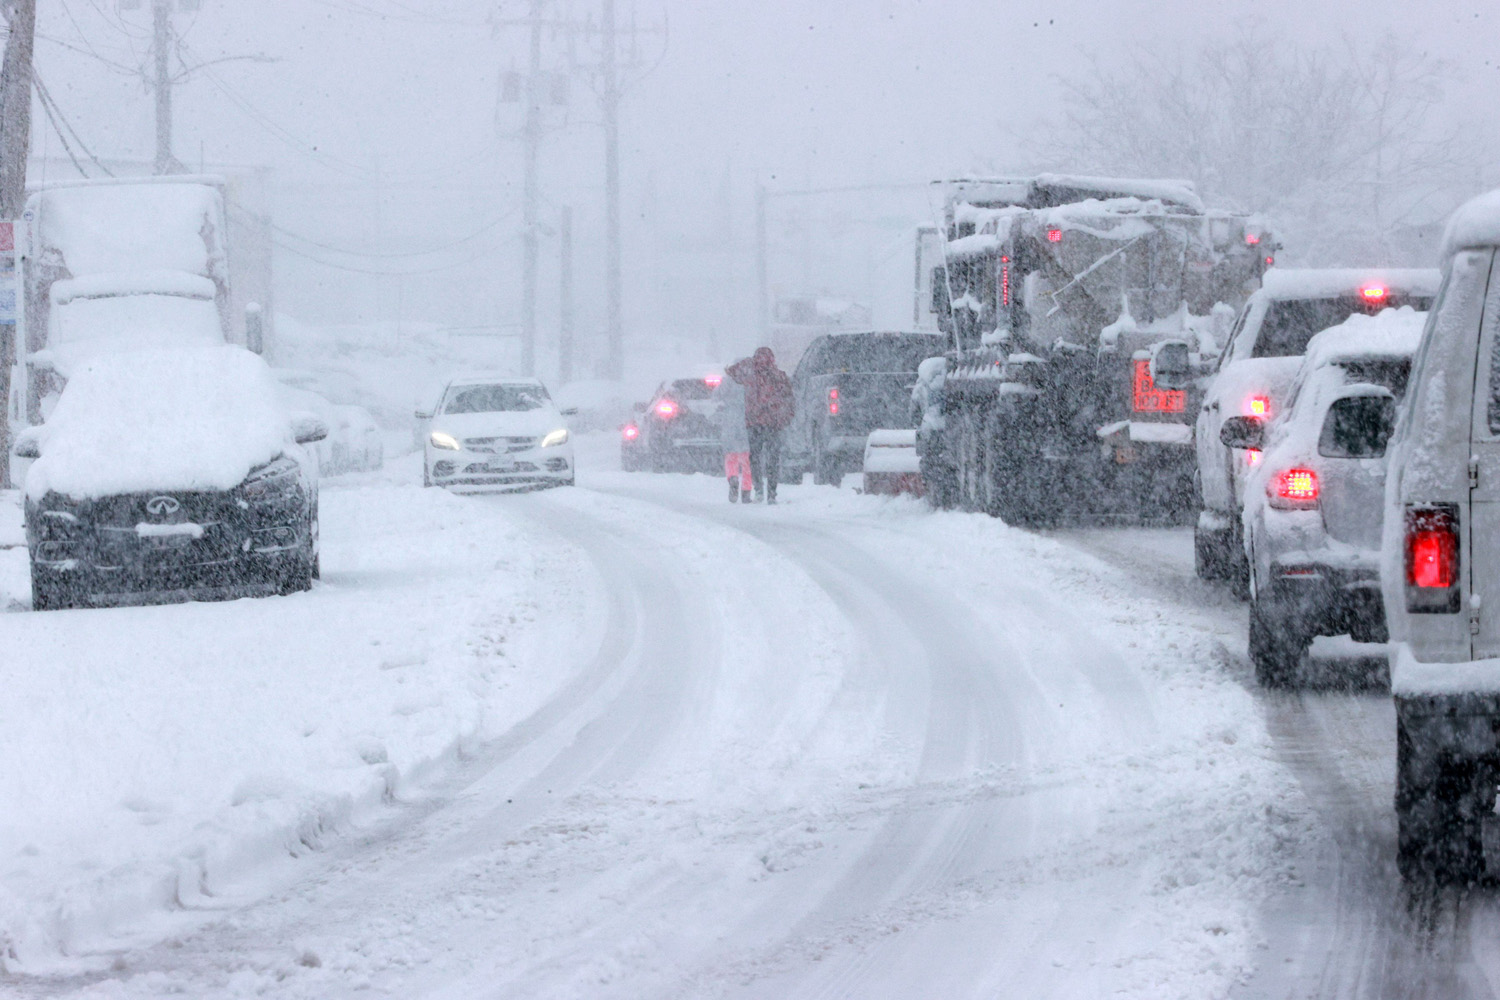
\includegraphics[width=0.6\textwidth]{Images/Illustration/ConditionDifficiles.jpg}
    \caption[]{Conditions typiques de fonctionnement du projet\footnotemark[1]}
    \label{ConditionDifficiles}
\end{figure}

\footnotetext[1]{Copyright: MediaPunch/Shutterstock}

\subsection{LoRaWAN}

LoRaWAN (acronyme de \emph{long-range wide-area network}) est un réseau de communication radio spécifique
à l'internet des objets (IoT). Ce protocole est utilisé pour transmettre des données sur des grandes 
distances tout en permettant une consommation électrique très faible. La longue portée de son signal 
permet d'installation d'appareils dans des endroits isolés, sans nécessairement avoir accès au réseau 
électrique ou mobile.\\
La topologie de LoRaWAN est dite en étoile d'étoiles. En effet, comme le montre la figure \ref{LoRaWANTopo},
le serveur d'application se trouve au centre, et les passerelles réparties sur un territoire donné 
communiquent avec les appareils installés.

\begin{figure}[H]
    \centering
    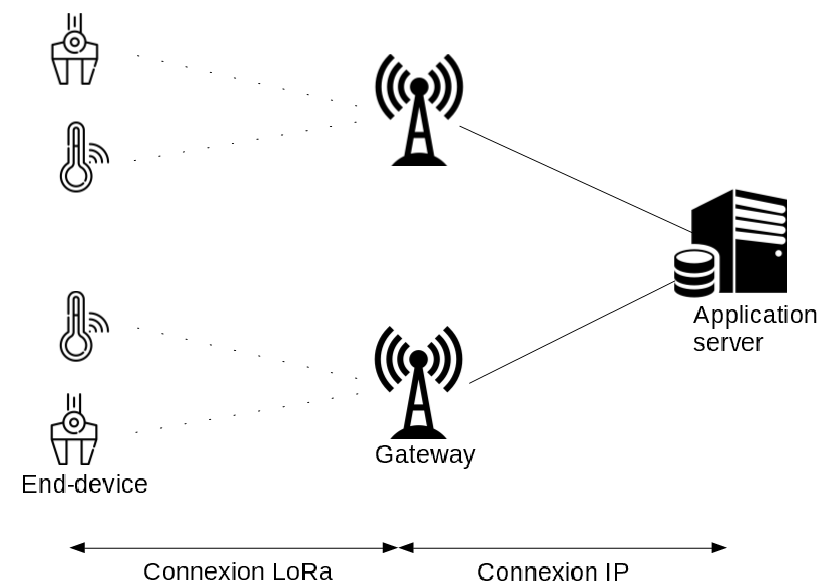
\includegraphics[width=0.6\textwidth]{Images/Illustration/Architecture_lorawan.png}
    \caption[]{Topologie LoRaWAN\footnotemark[1]}
    \label{LoRaWANTopo}
\end{figure}

\footnotetext[1]{Tiré de la page Wikipedia LoRaWAN}

\subsection{Edge Computing}

Comme le réseau LoRa utilisé permet une transmission de donnée bas débit, il est important d'économiser
le plus possible la bande passante. Pour cela, la méthode d'optimisation d'\emph{Edge Computing} est
privilégiée, rapprochant le traitement des données au plus proche des capteurs.\\
En pratique, dans ce projet, cela signifie que les données récoltées seront traitées directement sur 
le module LoRaSnow. Ainsi, uniquement les résultats des mesures seront envoyées dans le cloud.

\subsection{Notre interprétation du cahier des charges}
Comme le cahier des charges donne un objectif à atteindre, nous avons jugé important de préciser les 
étapes à accomplir pour détecter de la neige sur une route.

\begin{description}
    \item[Mesure de hauteur de neige] \hfill \\ 
    Afin d'avoir une indication sur l'enneigement de la route, nous 
    avons trouvé utile d'avoir une information sur la hauteur de neige présente dans le but d'avoir 
    une vue global d'une région grâce à un réseau de capteurs. Sur un vaste territoire comme certaines
    communes de montagne, l'enneigement peut être irrégulier. De cette manière, nous pouvons connaître 
    facilement l'état des routes dans des endroits isolés.
    \item[Reconnaissance du débit de neige et de l'état de la route] \hfill \\
    En plus des informations de hauteur de neige, nous avons couplé une solution de vision par ordinateur
    qui nous permet de récolter des mesures sur l'enneigement de la route ainsi que le débit actuel de
    flocons, dans l'objectif de faire des prévisions à court terme.\\
    Nous avons estimé qu'il était important de créer une redondance sur l'indication de l'état de la
    route. En effet, nous nous attendons à ce que la mesure physique de hauteur de neige ne soit pas 
    capable de donner des résultats pertinents pour les premiers millimètres.
    \item[Fixation et protection du module] \hfill \\ 
    Comme le module LoRaSnow sera exposé au aléas météorologiques de la montagne, un boitier étanche 
    et résistant doit être confectionné. Il doit permettre de protéger totalement l'électronique de 
    l'humidité et d'autres types de perturbations. Il offre aussi un collier de fixation pour permettre 
    une installation facile et fiable. L'élévation du module doit aussi être réglable.
\end{description}

L'avantage principal de ce cahier des charges explicite résite dans le fait qu'il est très facile pour
nous de séparer les tâches entre les collaborateurs du projet. Ainsi, chaque solution n'est que très 
peu couplée les unes par rapport aux autres durant le prototypage.

\section{Schéma bloc global}

\begin{figure}[H]
    \centering
    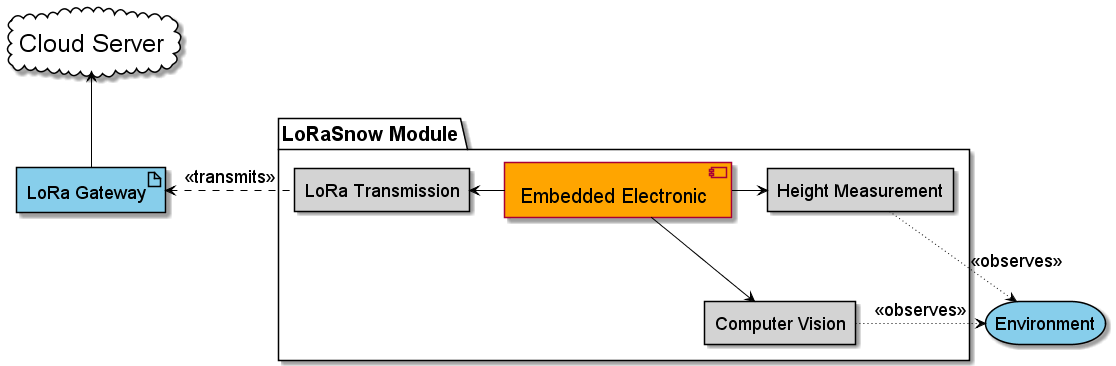
\includegraphics[width=0.9\textwidth]{Diagram/out/Diagram/BlockDiagram/GlobalBlockDiagram.png}
    \caption{Schéma bloc global du projet}
    \label{GlobalBlockDiagram}
\end{figure}

\begin{description}
    \item[\emph{Environment}] \hfill \\ 
    Ceci représente l'environnement mesuré, c'est-à-dire la route enneigée. Il est important de noter
    que les deux capteurs qui observent l'environnement le font de manière non-intrusive.
    \item[\emph{Height Measurement}] \hfill \\
    Ce capteur se charge de mesurer une hauteur de neige sur la route selon une méthode définie. Il 
    communique ses mesures directement à l'élément central du projet. 
    \item[\emph{Compteur Vision}] \hfill \\
    Cette partie s'occupe de mesurer le débit de flocons et sert de complément à la partie de mesure 
    de hauteur. 
    \item[\emph{Embedded Electronic}] \hfill \\
    L'électronique embarquée représente la partie central du projet. C'est ici que l'on retrouve le
    microcontrôleur qui traiter les données reçues par les différents capteur et de transmettre les
    résultats. 
    \item[\emph{LoRa Transmission}] \hfill \\
     Le module de transmission LoRa reçoit les données du microcontrôleur et les envoie sur le réseau 
     LoRaWAN à l'aide d'une antenne à l'intérieur du boitier.
    \item[\emph{LoRa Gateway}] \hfill \\
    La passerelle LoRaWAN couvre une surface donnée dans laquelle se trouvent un ou plusieurs modules 
    LoRaSnow. Ainsi, les données transmises sont réceptionnées et retransmises sur un réseau IP. 
    \item[\emph{Cloud Server}] \hfill \\   
    Finalement, on retrouve un serveur dans le cloud se chargeant de la bonne réception des données 
    de tous les modules LoRaSnow d'un même groupe. Les données récoltées peuvent ainsi être mise en
    forme et utilisées pour indiquer par exemple la couverture neigeuse d'une région.
\end{description}

Les trois derniers points évoqués n'ont pas encore été implémentés dans le projet.